\chapter{Contexte général}

\section*{Introduction}

Ce chapitre présente le contexte général du projet CrediWise. Il introduit l'entreprise d'accueil IntechGeeks, décrit le secteur de la microfinance en Tunisie, qui motive le projet, analyse les points forts et les limites de la solution existante DigiLAF, présente la plateforme CrediWise proposée et expose la méthodologie Scrum adoptée pour le développement.

\section[Organisme d'accueil]{Organisme d'accueil}

\subsection{Présentation d'IntechGeeks}

IntechGeeks est une société d'ingénierie et d'intelligence artificielle au service de clients en Europe et en Afrique. Ses activités couvrent l'architecture logicielle cloud-native, l'intégration de systèmes et l'intelligence artificielle appliquée, avec un accent particulier sur la modernisation des systèmes d'information organisationnels. La figure~\ref{fig:intech} présente le logo de l'entreprise.

\begin{figure}[H]
    \centering
    
\includegraphics[width=0.3\textwidth]{img/intech.png}
    \caption{Logo d'IntechGeeks}
    \label{fig:intech}
\end{figure}

\subsection{Valeurs fondamentales}

Le travail de l'entreprise s'articule autour de principes qui guident la collaboration et la réalisation technique :

\begin{itemize}
    \item \textbf{Rigueur technique :} Les systèmes livrés sont testés, documentés et instrumentés. Les tests automatisés, les pipelines reproductibles et l'observabilité sont considérés comme des critères essentiels de qualité du projet.

    \item \textbf{Immersion avant exécution :} Avant le début du développement, l'entreprise analyse le contexte opérationnel du client, les systèmes existants, les contraintes et les flux de travail, afin que la solution proposée corresponde aux besoins réels de l'entreprise.

    \item \textbf{Transfert de connaissances :} La livraison du projet comprend une documentation, l'explication des choix techniques et un accompagnement destiné à aider les équipes clientes à exploiter la solution livrée.

    \item \textbf{Transparence :} L'avancement du projet, les décisions techniques et les risques identifiés sont communiqués aux parties prenantes tout au long de la mission.
\end{itemize}

\subsection{Structure organisationnelle}

La figure~\ref{fig:structure_org} illustre la structure organisationnelle d'IntechGeeks.

\begin{figure}[H]
    \centering
    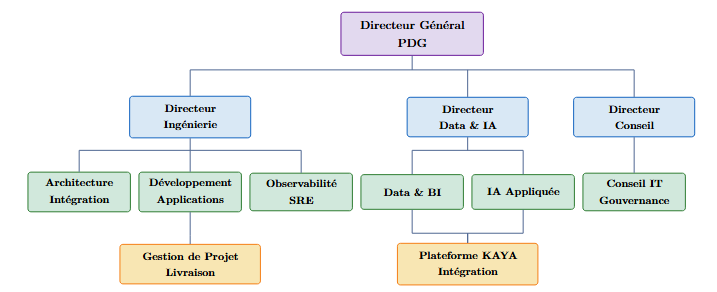
\includegraphics[width=0.85\textwidth]{img/Structure Organisationnelle.png}
    \caption{Structure organisationnelle d'IntechGeeks}
    \label{fig:structure_org}
\end{figure}

\section{Présentation du sujet}

Ce projet de fin d'études porte sur la conception et le développement de \textbf{CrediWise},
une plateforme web de gestion du crédit. L'objectif est de digitaliser et sécuriser
l'ensemble du cycle de vie du crédit, de l'entrée en relation client jusqu'à la décision
finale et la traçabilité.

\section{Étude de l'existant}

La gestion des demandes de crédit au sein des institutions de microfinance en Tunisie
s'inscrit dans un contexte de transformation numérique progressive. C'est dans ce cadre
que la solution \textbf{DIGILAF} a été développée, avec pour ambition de digitaliser et
de structurer l'intégralité du cycle de traitement des dossiers de crédit, depuis la
soumission de la demande jusqu'au décaissement des fonds.

\subsection*{\ding{226}~La solution DIGILAF}

DIGILAF est une solution métier dédiée aux institutions de microfinance et aux banques de
détail. Elle vise à :

\begin{itemize}
    \item accroître l'efficacité opérationnelle et commerciale des équipes de traitement ;
    \item standardiser le processus d'octroi de crédit à travers un workflow structuré et
    contrôlé ;
    \item maintenir un portefeuille de crédit sain grâce à une évaluation rigoureuse des
    dossiers ;
    \item garantir la traçabilité des décisions à chaque étape du cycle de vie d'une
    demande.
\end{itemize}

\subsection*{\ding{226}~Implémentation actuelle}

L'application en production repose sur \textbf{Microsoft Power Apps} en mode
\textbf{Canvas App}, une plateforme low-code/no-code permettant la création rapide
d'applications métier. Elle a été déployée pour remplacer des processus entièrement pilotés
sous Excel, avec pour objectif de moderniser la gestion des dossiers de crédit sans
mobiliser d'importantes ressources de développement logiciel.

\subsection*{\ding{226}~Fonctionnalités couvertes}

L'application prend en charge l'ensemble du cycle de traitement à travers les étapes
suivantes :

\begin{figure}[H]
    \centering
    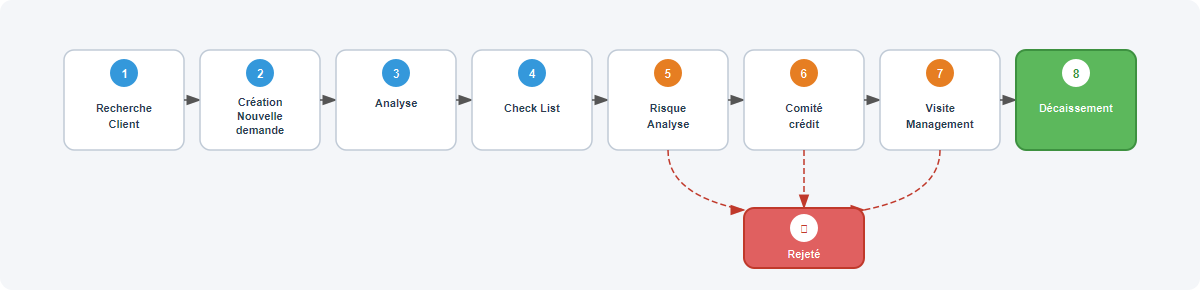
\includegraphics[width=0.95\textwidth]{img/process-steps.png}
    \caption{Étapes du processus de traitement des dossiers de crédit — DIGILAF}
    \label{fig:process_steps}
\end{figure}

Les transitions entre les différentes étapes sont partiellement automatisées via
\textbf{Power Automate}, qui assure la mise à jour des statuts des demandes ainsi que
l'envoi de notifications aux utilisateurs concernés.

\subsection*{\ding{226}~Gestion des accès et des rôles}

La répartition des responsabilités est gérée à travers le système de rôles de sécurité
de la \textbf{Microsoft Power Platform}. Chaque utilisateur dispose d'un périmètre d'accès
défini en fonction de son rôle dans le processus de traitement, garantissant que chaque
étape est prise en charge par l'intervenant habilité.

\section{Problématique}

Bien que DIGILAF ait constitué une avancée significative par rapport aux pratiques manuelles
basées sur Excel, l'analyse de la solution existante révèle plusieurs limitations
structurelles qui freinent son évolution et compromettent sa capacité à répondre aux
exigences croissantes des institutions financières :

\begin{itemize}
    \item \textbf{Restrictions de personnalisation :} Power Apps impose des contraintes
    importantes sur la conception des interfaces utilisateur, limitant la possibilité
    d'offrir une expérience ergonomique et adaptée aux besoins métier spécifiques ;
    \item \textbf{Limitation du volume de données :} la connexion à SQL Server est
    plafonnée à 2\,000 lignes par requête, ce qui constitue un obstacle majeur pour les
    institutions gérant un volume important de dossiers clients ;
    \item \textbf{Problèmes de performance :} à mesure que la complexité de l'application
    et le volume des données augmentent, des ralentissements significatifs sont observés,
    affectant la productivité des équipes ;
    \item \textbf{Dépendance à l'éditeur :} les mises à jour majeures de Power Apps peuvent
    impacter les fonctionnalités existantes, exposant la solution à des dysfonctionnements
    ou interruptions imprévus sans maîtrise du code source ;
    \item \textbf{Coût des licences :} l'exploitation de Power Apps nécessite des licences
    payantes par utilisateur, représentant une charge financière récurrente qui limite
    l'extension de la solution à un plus grand nombre de collaborateurs.
\end{itemize}

L'ensemble de ces contraintes rend la solution actuelle insuffisante pour accompagner
efficacement la montée en charge et les ambitions de transformation numérique des
institutions de microfinance.

\section{Solution proposée}

Afin de répondre aux limitations identifiées et d'accompagner la croissance des institutions
de microfinance, \textbf{CrediWise} est développé comme une refonte complète de la solution
DIGILAF. Il ne s'agit pas d'une simple amélioration de l'existant, mais d'une réécriture
intégrale reposant sur des technologies modernes, ouvertes et conçues pour garantir la
pérennité du système.

\subsection*{\ding{226}~Une architecture pensée pour la scalabilité}

CrediWise adopte une architecture à microservices dans laquelle chaque étape du cycle de
crédit est prise en charge par un service indépendant : Gestionnaire, Client, Nouvelle
Demande, Analyse, Checklist, Analyse des risques, Comité de crédit et Décaissement. Chaque
service dispose de sa propre base de données PostgreSQL conformément au patron
\textit{Database per Service}, garantissant l'isolation des responsabilités, une meilleure
maintenabilité et une grande capacité de montée en charge.

\subsection*{\ding{226}~Une indépendance vis-à-vis des éditeurs tiers}

Contrairement à Power Apps, CrediWise repose entièrement sur des technologies open source
telles que Quarkus, React, PostgreSQL et Keycloak. Ce choix offre une maîtrise complète du
code source et réduit la dépendance à des plateformes propriétaires, tout en limitant les
risques liés aux changements de licences ou aux évolutions imposées par des éditeurs tiers.

\subsection*{\ding{226}~Une expérience utilisateur moderne et personnalisable}

L'interface utilisateur, développée avec React et TypeScript, est entièrement personnalisable
afin de répondre aux besoins métier de l'institution. Elle s'appuie sur un mécanisme de
contrôle d'accès basé sur les rôles via Keycloak, garantissant que chaque acteur du
processus — Front Office, CRO, Analyste Risque, Décideur Agence ou Décideur Siège — accède
uniquement aux fonctionnalités correspondant à ses responsabilités.

\subsection*{\ding{226}~L'intelligence artificielle au service de la décision de crédit}

CrediWise intègre un module de recommandation basé sur l'intelligence artificielle, capable
d'analyser les données d'un dossier de crédit et de proposer une recommandation argumentée.
Cet outil assiste les analystes dans leur processus d'évaluation sans se substituer à leur
jugement, contribuant ainsi à améliorer la cohérence des décisions et à réduire les délais
de traitement.

\subsection*{\ding{226}~Une observabilité et une traçabilité complètes}

L'ensemble des services est instrumenté à l'aide d'OpenTelemetry et supervisé via SigNoz.
Cette infrastructure permet de suivre les performances de la plateforme, de surveiller les
flux de traitement et de détecter rapidement les anomalies éventuelles, offrant ainsi un
niveau de visibilité absent de la solution existante.

Ainsi, CrediWise constitue une réponse cohérente et durable aux limites identifiées dans
DIGILAF, en mettant l'accent sur la performance, l'évolutivité, la maîtrise technologique
et l'amélioration de l'expérience utilisateur.


\section{Méthodologie adoptée}

La réussite d'un projet informatique repose sur une méthodologie de travail structurée.
Celle-ci permet d'organiser les activités, de respecter les délais et de garantir la qualité
des livrables tout au long du cycle de développement.



\subsection{Choix de la méthodologie de travail}

Pour assurer une gestion efficace du projet, nous avons adopté la méthodologie
\textbf{Agile Scrum}~\cite{BocasayScrum}. Cette approche permet une organisation du travail
en sprints, favorise la livraison progressive des fonctionnalités et facilite l'adaptation
aux évolutions des besoins. Elle offre également une meilleure visibilité sur l'avancement
du projet, tout en impliquant régulièrement les parties prenantes dans le processus de
développement.

\subsection{Répartition des rôles}

Une équipe Scrum est composée du Product Owner, du Scrum Master et de l'équipe de
développement. Ces rôles complémentaires collaborent afin d'assurer le bon déroulement
du projet et la livraison régulière de fonctionnalités à valeur ajoutée.

\subsubsection{Scrum Master}

Le Scrum Master veille à l'application des principes Scrum et accompagne l'équipe dans
leur mise en œuvre. Il facilite la communication et contribue à la résolution des obstacles
rencontrés durant le projet.

\subsubsection{Product Owner}

Le Product Owner est responsable de la gestion du Product Backlog et de la priorisation
des besoins. Il assure la liaison entre les parties prenantes et l'équipe de développement
afin de garantir l'adéquation de la solution aux besoins métier.

\subsubsection{Équipe de Développement}

L'équipe de développement regroupe les membres chargés de concevoir, développer et tester
la solution. À chaque sprint, elle produit un incrément fonctionnel respectant les critères
de qualité définis.

\subsubsection{Les événements de Scrum}

La méthodologie Scrum repose sur plusieurs événements permettant de suivre l'avancement
du projet :

\begin{itemize}
    \item \textbf{Sprint Planning :} définition des objectifs et des tâches du sprint.
    \item \textbf{Daily Scrum :} réunion quotidienne de suivi et de coordination.
    \item \textbf{Sprint Review :} présentation et validation des fonctionnalités réalisées.
    \item \textbf{Sprint Retrospective :} identification des améliorations à apporter aux
    prochains sprints.
    \item \textbf{Backlog Refinement :} clarification et estimation des éléments du
    Product Backlog.
\end{itemize}

\begin{figure}[H]
    \centering
    
\includegraphics[width=0.85\textwidth]{Scrum.png}
    \caption{Cycle de vie SCRUM}
    \label{fig:scrum_lifecycle}
\end{figure}

\section*{Conclusion}

Ce chapitre débute par une présentation de l'organisme d'accueil. Par la suite, nous avons
exposé une vue globale du projet, incluant la description de la solution actuelle, ses limites,
la problématique identifiée, ainsi que la solution envisagée. Enfin, nous avons expliqué la
méthodologie de gestion de projet adoptée. Le chapitre suivant se focalisera sur l'analyse
et la spécification des besoins du projet.
